\documentclass[11pt,a4paper]{article}
\usepackage{amsmath}
\usepackage{amssymb}
\usepackage{graphicx}
\usepackage{verbatim}
\begin{document}
\noindent
Martin Lundfall, Henri Bunting, Malte Siemers, Patrik Bey
\begin{centering}
  \section*{Exercise sheet 09 - Machine Intelligence I}
  \end{centering}
\section*{9.1}
The primal problem for C-SVMs is solved by using the Karush-Kuhn-Tucker conditions, a generalization of Lagrange multipliers. We aim to minimize the following equation:
\begin{equation}
  L_{(w, b, \{\lambda_\alpha\})} = f_0(w, b) + \sum_{\alpha=1}^p \lambda_\alpha f_\alpha(x)
\end{equation}
Where $f_0$ is the function to be minimized, in our case:
\begin{equation}
f(w,b) = \frac{||w||^2}{2} + \frac{C}{p}\sum_{\alpha=1}^p \varphi_\alpha
\end{equation}
 and $f_k$ are the inequality constraints, in our case:
\begin{equation}
f_\alpha(w, b) = (1 - \varphi_\alpha) - y_T (w^Tx + b)
\end{equation}
\begin{equation}
f_\alpha(w, b) = - \varphi_\alpha
\end{equation}
We minimize the KKT equation first with respect to $w$. Note that the slack variables $\varphi_\alpha$ are independent of $w$. This results in:
\begin{equation}
w = \sum_{\alpha=1}^p \lambda_\alpha y_T^{(\alpha)}x^{(\alpha)}
\end{equation}
Then minimizing with respect to $b$ we get the following constraint on $\lambda_\alpha$:
\begin{equation}
0 = \sum_{\alpha=1}^p \lambda_\alpha y_T^{(\alpha)}
\end{equation}
Putting these results back into the KKT equation, we attain:
\begin{equation}
L_{(x_k, \{\lambda_k\})} = \frac{1}{2} \sum _{\alpha, \beta=1}^p\lambda_\alpha \lambda_\beta y_T^{(\alpha)}y_T^{(\beta)}(x^{(\alpha)})^Tx^{(\beta)}+\sum_{\alpha=1}^p\lambda_\alpha
\end{equation}
We clearly see that minimizing this equation corresponds to maximizing the expression given in the exercise. The upper bound of the $\lambda_\alpha$ variables is given by the duality of the problem.

\section*{9.4 - Parameter Optimization}
\subsection*{(a)}
Following the procedure for grid search as described in the guide we performed leave-one-out cross validation (LOOCV) on the training data using the following parameter range:\\
$ \gamma = [2^{3},2,2^{-1},2^{-3},2^{-5},2^{-7},2^{-9}] $, $ C = [2^{-5},2^{-3},2^{-1},2,2^{3},2^{5},2^{7}]$

\begin{figure}[h]
	\includegraphics[width=\linewidth]{train_dat_model.jpg}
	\caption{Example SVM model for the given training data}
\end{figure}

\subsection*{(b)}
The following contour plot shows the classification performance for LOOCV on the training data with the parameter grid as defined in \textbf{(a)}.

\begin{figure}[h]
	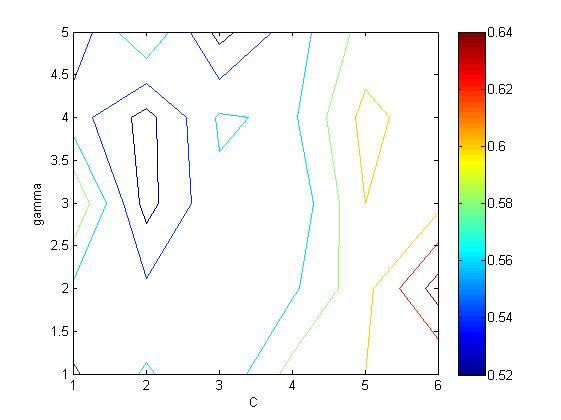
\includegraphics[width=\linewidth]{perf_contour.jpg}
	\caption{Contour plot for the given LOOCV performances for each combination of $C$ and $\gamma$}
\end{figure}

\newpage
\subsection*{(c)}
The optimal parameter values for $C$ and $\gamma$ given the LOOCV on the training data are
$C = 2^{3}, \gamma = 2^{-9}$ for an overall LOOCV performance of $97.5\%$.

\subsection*{(d)}
The following plot shows the test data and the decision boundary for a trained SVM given the optimal parameter as given in \textbf{(c)}.
\begin{figure}[h]
	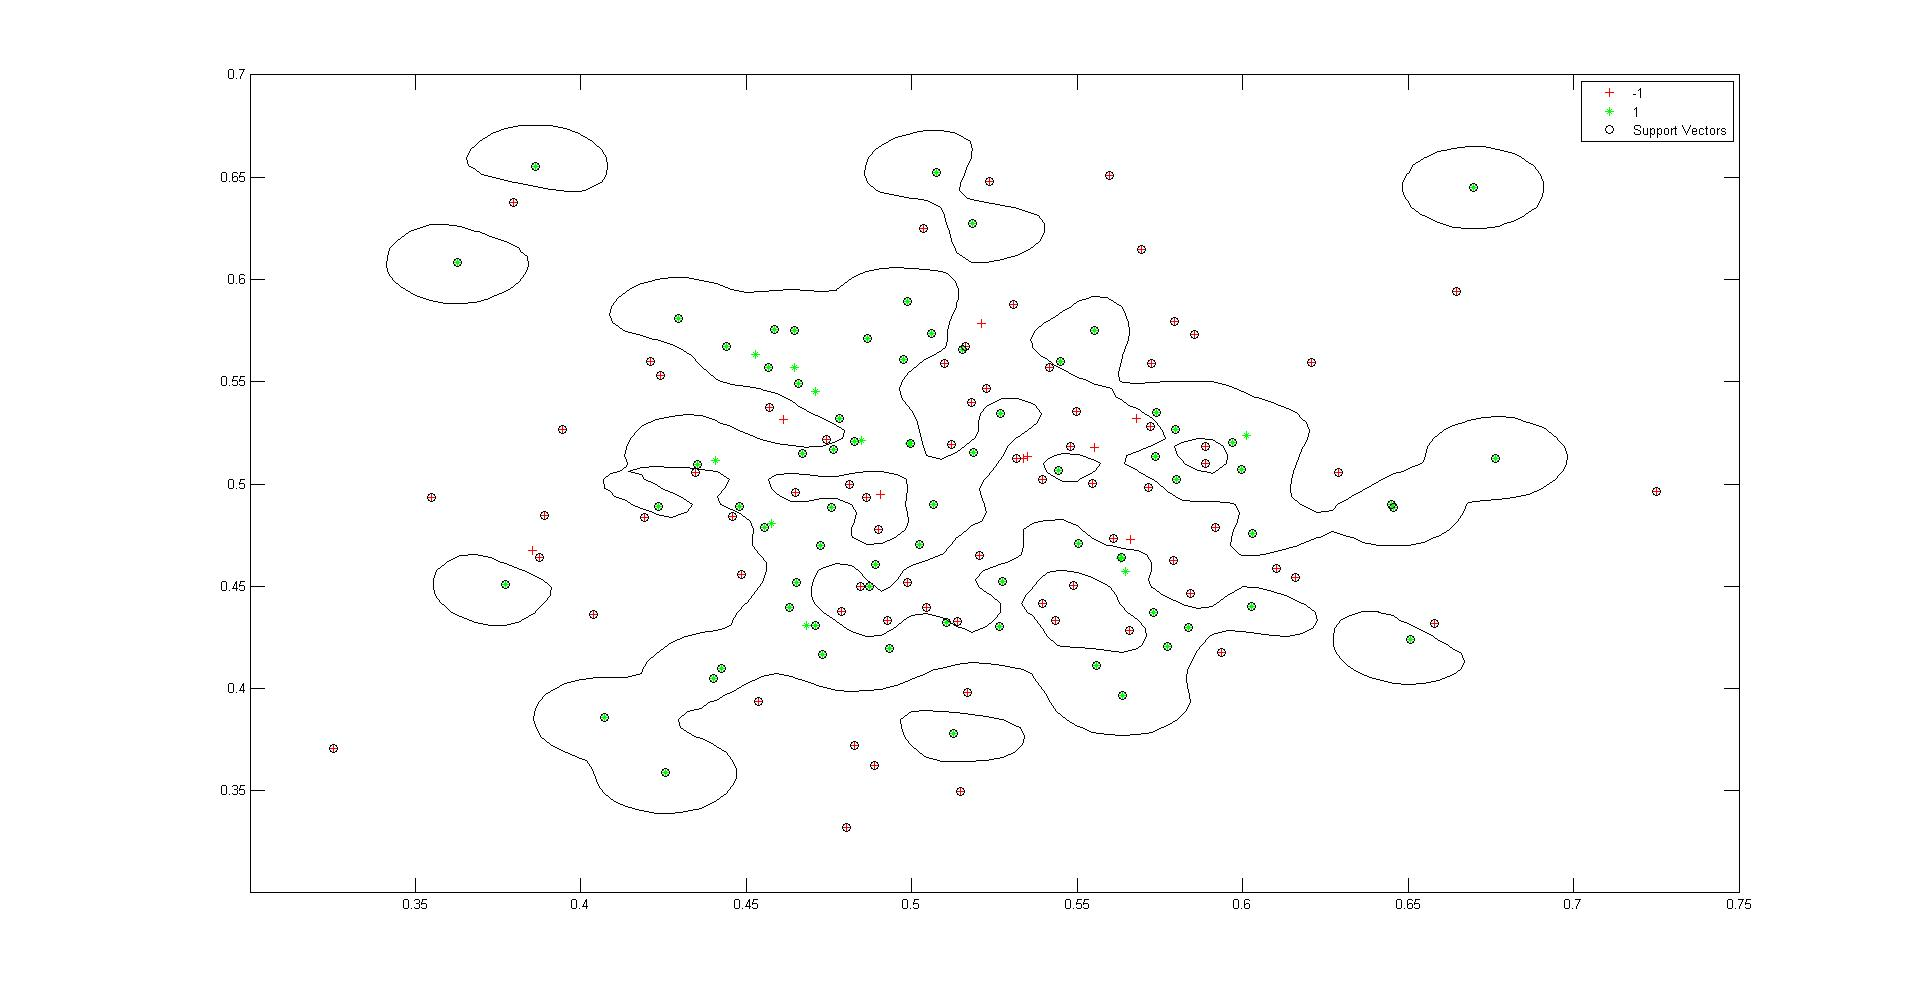
\includegraphics[width=\linewidth]{test_dat_model.jpg}
	\caption{Classification of test data based on optimal parameter from grid search on training data}
\end{figure}

\subsection*{(e)}
The grid search over the parameters $C$ and $\gamma$ enables the trained machine to construct a decision boundary which is more adjust towards the exact position of the training data points. This bears the risk of over-fitting which can be seen in the plot in \textbf{(e)} by the total amount of support vectors (circles).

\end{document}
